\section{Facit}

\begin{opgave}{Hubbleloven}
    \opg Hubbleloven beskriver universets udvidelse, der får alting til at bevæge sig væk fra hinanden. Negative hastigheder betyder at himmellegemer bevæger sig imod os, hvilket ikke kan skyldes universets udvidelse. Ergo gælder Hubbleloven kun for objekter med $v > 0$. Hvis man prøvede alligevel ville man få en negativ længde, og det giver ikke mening.
    \opg Lys bliver blåforskudt, når lyskilden bevæger sig imod modtageren. Af spørgsmål \textbf{1}) gælder Hubbleloven derfor ikke.
\end{opgave}

\begin{opgave}{Den kritiske tæthed}
\opg Hvis universet er fladt har det ingen krumning, hvorfor $\kappa = 0$
\opg Indsættes $\kappa = 0$ i Friedmannligningen fås
%
\begin{align*}
    H^2 &= \frac{8\pi G \rho}{3} + \frac{\Lambda}{3}, \\
    \implies H^2 - \frac{\Lambda}{3} &= \frac{8\pi G}{3}\rho.
\end{align*}
%
Ganges brøken over fås
%
\begin{align*}
    \rho_c = \frac{1}{8\pi G}\left(3H^2 - \Lambda\right).
\end{align*}
%
\opg $\Lambda \ll 3H^2 \implies 3H^2 - \Lambda \simeq 3H^2$ hvorfor
%
\begin{align*}
    \rho_c \simeq \frac{3H_0^2}{8\pi G}.
\end{align*}
%
\opg Bruges værdierne $H_0 = \SI{67.7}{\kilo\meter\per\second\per\mega\parsec}$ og $G = \SI{6,6742e-11}{\newton\square\metre\per\square\kilo\gram}$ fås
%
\begin{align*}
    \rho_\text{c} \simeq \frac{3H_0^2}{8\pi G} = \frac{3(\SI{67.7}{\kilo\meter\per\second\per\mega\parsec})^2}{8\pi\cdot\SI{6,6742e-11}{\newton\square\metre\per\square\kilo\gram}} =  \SI{8.6e-27}{\kilo\gram\per\cubic\metre}.
\end{align*}
\end{opgave}

\begin{opgave}{Et univers af bolde}
\opg Isoleres $n_\mathrm{b}$ i ligning \eqref{eq:antalsdensitet} og indsættes værdierne $m_\mathrm{b} = \SI{1}{M_\odot}$ og $\rho_\text{c} = \SI{8.6e-27}{\kilo\gram\per\cubic\metre}$ fås
%
\begin{align*}
    n_\mathrm{b} = \frac{\rho_\mathrm{c}}{m_\mathrm{b}} = \frac{\SI{8.6e-27}{\kilo\gram\per\cubic\metre}}{\SI{1}{M_\odot}} = \SI{4,3e-57}{\per\cubic\metre}.
\end{align*}
\opg Indsættes ovenstående resultat fås
%
\begin{align*}
    d_\mathrm{b} = n_\mathrm{b}^{-1/3} = (\SI{4,3e-57}{\per\cubic\metre})^{-1/3} = \SI{198.9}{\parsec}.
\end{align*}
\opg Indsættes værdierne $d_\mathrm{b} = \SI{198.9}{\parsec}$, $H_0 = \SI{67.7}{\kilo\meter\per\second\per\mega\parsec}$ og $\si{\clight} = \SI{2.99792e8}{\metre\per\second}$ fås
%
\begin{align*}
    \frac{d_\mathrm{max}}{d_\mathrm{b}} = \frac{\si{\clight}/H_0}{d_\mathrm{b}} = \frac{\SI{2.99792e8}{\metre\per\second}/\SI{67.7}{\kilo\meter\per\second\per\mega\parsec}}{\SI{198.9}{\parsec}} = \SI{2.2e7}{}.
\end{align*}
\opg Denne delopgave kan ikke løses, da størrelsen af boldene ikke er oplyst. Hvis den var, kunne man beregne sandsynligheden for at en foton i en given retning fra os vil ramme en bold inden for en bestemt radius. Det gøres ved at for hver kugleskal af himlen i en bestemt radius fra os, og med en lille tykkelse dx, kan man finde et gennemsnitligt antal bolde, da vi kender deres tæthed. Sandsynligheden for at en foton bliver stoppet i denne kugleskal, er så arealet dækket af bolde divideret med det totale areal. Man kan integrere over disse kugleskaller, for at finde den totale sandsynlighed for at blive stoppet inden for en radius $s$, som man integrerer ud til (ligesom i eksemplet med Olbers paradoks). Så spørgsmålet kan omformuleres til: Hvad er sandsynligheden for at en fotons bane fra os brydes inden radius $d_{max}$, antaget en bestemt boldradius $r$? %Det kosmologiske princip siger, at universet er homogent og isotropt -- altså at massen er jævnt fordelt over hele universet, og at det ser ens ud i alle retninger. Hvis vi skal kunne se noget i afstanden $d_\mathrm{max}$ i et univers kun bestående af bolde, så skal der være et retning, hvor den nærmeste bold er i den afstand. Skal man kunne se cirka 22 millioner gange længere end den gennemsnitlige afstand mellem bolde, så svarer det løst sagt til at der mangler 22 millioner bolde i en bestemt retning, og de må jo så være et andet sted i universet. Det ville dog betyde at der er forskel på hvilken retning vi kigger i, og at massetætheden ikke er den samme alle steder. Det er derfor usandsynligt, at have et univers bestående af sådanne ens bolde, hvor universet har den nuværende massetæthed, hvor vi kan se noget i afstanden $d_\mathrm{max}$, mens det kosmologiske princip er gældende. Det er ikke direkte i modstrid med det kosmologiske princip, da \SI{2,2e7}{M_\odot} ikke er voldsomt stort på kosmologisk skala -- til sammenligning er massen af mælkevejen $\sim \SI{1e12}{M_\odot}$ -- men det er stort nok til at være betydningsfuldt.
\opg Denne delopgave kan ikke løses, da størrelsen af boldene ikke er oplyst. %Hele udregningen byggede på en antagelse om at universet kun består af består af bolde med massen $m_\mathrm{b} = \SI{1}{M_\odot}$. Denne antagelse har svært ved at forklare den afstand vi kan se i universet, hvorfor der må være noget galt med antagelsen. Det mest oplagte er tyngdekraften får masse til at klumpe sig sammen til objekter, der er tungere end 1 solmasse. Dette ses også ved den markante forbedring af $d_\mathrm{max}/d_\mathrm{b}$ ved at bruge Mælkevejens masse. På stor skala er Universet altså bedre beskrevet som en samling af ens galakser end en samling af ens stjerner. Dette viser også at det kosmologiske princip fungerer på store længde skalaer, men ikke på mindre. Det er eksempelvis ikke sandt, at alle dele af Mælkevejen ser ens ud fra Jorden -- der er langt mere masse, hvis vi kigger mod galaksens centrum, end hvis vi kigger i den modsatte retning. Galakser samler sig også i galaksehobe, og bruges massen for sådan en fås, at vi kan se cirka 200 gange længere end den gennemsnitlige afstand mellem bolde i et univers hvor boldene vejer det samme som en galaksehob. Dette tyder på, at universet skal det beskrives på en skala af galakser og galaksehobe. Modellen tager ikke højde for at boldene kan have forskellig masse og derudover er synslængde ikke nok i sig selv til at kunne afgøre om modellen er brugbar. Det virker dog sandsynligt, at Universet på tilpas stor skala opfører sig som en samling af galakser og galaksehobe, da det kosmologiske princip lægger op til, at en model med ens bolde ikke er helt ved siden af.
\end{opgave}

\begin{opgave}{Dopplerforskydning}
	\opg 
	\begin{figure}[h!]
		\centering
		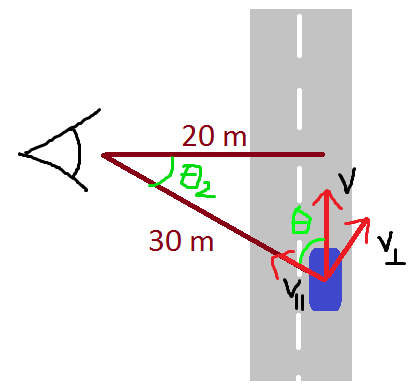
\includegraphics[width=0.5\textwidth]{opg/figurer/PolitiLoesning.png}
		%\caption{Et typisk } %https://upload.wikimedia.org/wikipedia/commons/9/98/Andromeda_Galaxy_%28with_h-alpha%29.jpg
	\end{figure}
	\opg Den radielle hastighed er den parallele komponent med synsvinklen. Vi ser en retvinklet trekant og bruger
	\begin{align}
		\cos(\theta)=\frac{\text{hosliggende katete}}{\text{hypotenusen}}=\frac{v_{radiel}}{v} \\
		v_{radiel}=v \cos(\theta)
	\end{align}
	Der dannes også en retvinklet trekant af vejen, afstanden til vejen og afstanden til bilen. I grader giver det en vinkel på
	\begin{align}
		\cos(\theta_2)&=\frac{20}{30}\\
		\theta_2 &= \cos^{-1} \left( \frac{20}{30} \right) = 48
	\end{align}
	De to vinkler indgår begge i en retvinklet trekant, så
	\begin{align}
		180 &= \theta + \theta_2 + 90\\
		\theta &= 90 - \theta_2  = 42
	\end{align}
	Vi indsætter og får
	\begin{align}
	v_{radiel}=50 km/t \cdot \cos(42) = 50 km/t \cdot 0.74 = 37 km/t
	\end{align}
	Hvis du ikke får det samme, så prøv at regne alt i radianer, da det er simplere.
	\opg 
	Du står stille, så $v_{kilde}=0$. $v_{obs}$ er den radielle hastighed, som lige skal omregnes til km/t:
	\begin{align}
	37 km/t = 37 \frac{10^{3}m}{60\cdot60 s} = \frac{37}{3.6} m/s = 10.3 m/s
	\end{align}
	Så indsætter vi i
	\begin{align}
	f_{obs} = \frac{340 m/s + 10,3}{340 m/s + 0} 800 Hz = 824 Hz
	\end{align}
    (Hz er enheden hertz, som er 1/s)
\end{opgave}

\begin{opgave}{Skalafaktor}
	Vi ved temperaturen dengang var $T(t) = 3000 K$ og nu er den $T_0 = 2.73 K$. Så vi kan bruge at skalafaktoren ændrer sig med rødforskydningen, og sammensætte det med hvordan den ændrer sig med temperatur:
	\begin{align}
	    a(t) = \frac{1}{1+z} = \frac{T_0}{T(t)}\\
	    z = \frac{T(t)}{T_0} - 1
	\end{align}{}
	Så vi kan nu regne fra temperatur til rødforskydning:
	\begin{align}
	    z = \frac{T(t)}{T_0} - 1 = \frac{3000 K}{2.73 K} - 1= 1,10\cdot10^3 -1 \approx 1,10\cdot10^3
	\end{align}
	Så der blev dannet atomer ved $z\approx1100$, da det blev koldt nok til elektroner kunne binde sig til atomkernenerne.
\end{opgave}

\begin{opgave}{Rødforskydning af kvasar}
	\opg nm er $10^{-9} m= 10 \cdot 10^{-10} m$, så H-$\alpha$-linjen er ved ca. $6560$ Å. På figur \ref{kvasar} er det ved omkring $7600$ Å, dvs. bølgelængden er blevet større, så lyset er rødforskudt. Altså må kvasaren bevæge sig væk fra os.\\
	\opg Den radielle hastighed er beskrevet af rødforskydningen. Rødforskydningen er
	\begin{align}
		\frac{\lambda_{obs}-\lambda_{lab}}{\lambda_{lab}} = \frac{7600-6560}{6560} = 0,159.
	\end{align}
	Det er lavt, så vi approksimerer hastigheden til
	\begin{align}
		v= z\cdot c = 0,159 \cdot 3\cdot 10^8 \frac{m}{s}= 4,7\cdot 10^7 \frac{m}{s}
	\end{align}
	Regner du det præcist, giver det nogenlunde det samme.
	\opg $\Delta\lambda \approx 200 Å$, så det giver $v=0.015 c = 4,5\cdot 10^6 m/s$.
\end{opgave}
\begin{opgave}{Afstande}
	\opg Isolér $D_M$ i hvert udtryk.
	\begin{align}
		D_M &= \frac{D_L}{1+z}\\
		D_M &= D_A(1+z)
	\end{align}
	Resultaterne sættes lig hinanden
		\begin{align}
		\frac{D_L}{1+z} &= D_A(1+z)\\
		D_L &= D_A (1+z)^2
		\end{align}
	\opg Ved $z=1$ er $D_C\approx3200 Mpc$ og derfor
	\begin{align}
		D_L &= D_M(1+z)= 3200 Mpc \cdot 2 = 6400 Mpc\\
		D_A &= \frac{D_M}{1+z}= 3200 Mpc/ 2 = 1600 Mpc.
	\end{align}
	Ved $z=9$ er $D_C\approx9200 Mpc$, så
	\begin{align}
		D_L &= D_M(1+z)= 9200 Mpc \cdot 10 = 92000 Mpc\\
		D_A &= \frac{D_M}{1+z}= 9200 Mpc/ 10 = 920 Mpc.
	\end{align}
	Gamle objekter, der har bevæget sig fra os længere tid, har altså en større luminositetsafstand, men en lavere vinkelafstand ved høje rødforskydninger. Man skulle ellers tro objekter så mindre ud på himlen, jo længere væk de var, hvilket er rigtigt indtil omkring $z=1,6$. I det tidlige univers var galakserne tættere på hinanden, så de fyldte meget på himlen for hinanden, og derfor er deres lys spredt ud over et stort område.
	\opg
	%Dengang var universet for resten kun 250 mio. år gammelt.\\
	Hvis vi approksimerer $z\approx\frac{v}{c}$, får vi overlyshastigheder, så det går ikke.
	\begin{align}
    	z+1&=\sqrt{\frac{1+\frac{v}{c}}{1-\frac{v}{c}}}\\
    	(z+1)^2&=\frac{1+\frac{v}{c}}{1-\frac{v}{c}}
	\end{align}
	så vi skal løse et system på formen $y=\frac{1+x}{1-x}$, hvor $y=(z+1)^2$ og $x=\frac{v}{c}$. Man kan omformulere det til $x=\frac{y-1}{y+1}$, ved
	\begin{align}
	    1+x &= y(1-x)\\
	    1+x &= y-yx \\
	    x+yx &= y-1 \\
	    x(1+y) &= y-1 \\
	    x &= \frac{y-1}{y+1}.
	\end{align}
    Derfor må
	\begin{align}
    	\frac{v}{c}&=\frac{(z+1)^2-1}{(z+1)^2+1}\\
    	v&=\frac{(z+1)^2-1}{(z+1)^2+1} c = \frac{(10+1)^2-1}{(10+1)^2+1} = 0.98 c. %3\cdot 10^{8} m/s =
	\end{align}
	Så svaret er 98 \% af lysets fart i vakuum.
\end{opgave}

\begin{opgave}{Andromeda-galaksen}
	\opg 
	\begin{align}
		D_H=\frac{v}{H_0} 
	\end{align}
	Vi skal bruge den radielle hastighed
	\begin{align}
		v \approx z c = -0.001 \cdot 3\cdot 10^8 m/s =-3\cdot 10^5 m/s
	\end{align}
	og omskriver Hubble-konstanten en lille smule
	\begin{align}
		H_0=70 km s^{-1} Mpc^{-1} = 7 \cdot 10^4 m s^{-1} Mpc^{-1}.
	\end{align}
	Vi indsætter
	\begin{align}
	D_H=\frac{-3\cdot 10^5 m s^{-1}} {7 \cdot 10^4 m s^{-1} Mpc^{-1}} = - 3/7 \cdot 10 Mpc = - 4.2 Mpc.
	\end{align}
	Så Hubble-afstanden bryder sammen og giver noget negativt. Ligesom i den første opgave, kan man ikke bruge Hubbles lov på negative rødforskydninger.
	
	\opg Vi omregner lysår (ly) til meter, så vi kan dividere med den radielle hastighed i m/s fra før og få en tid:
	\begin{align}
		2.5\cdot 10^6 ly = 2.5\cdot 10^6 \cdot 9.46 \cdot 10^{15} m = 23.7 \cdot 10^{21} m\\
		\frac{23.7 \cdot 10^{21} m}{3\cdot 10^5 m/s} = 7.9 \cdot 10^{16} s = 2.5 \cdot 10^9 yr
	\end{align} 
	Så det vil tage 2,5 mia. år, hvis vi ser bort fra accelerationen og andre effekter.
	Stjernerne ligger meget spredt i begge galakser, så det er ekstremt usandsynligt at vi kommer til at støde ind i andre - men det kan sagtens være solsystemet bliver slynget langt ud eller måske helt væk fra galakserne (så udsigten ændres men derudover betyder det ikke så meget for os). Når gassen fra galakserne kolliderer varmes det op, og vi vil derfor se en masse ny stjernedannelse. Galakserne vil med tiden smelte sammen til en elliptisk galakse, der har opbrugt det meste gas, så stjernedannelsen stopper.
\end{opgave}